% <-- a percent symbol indicates a comment which does not affect the output of LaTeX
% you can leave the preamble alone, from here ...
\documentclass[12pt]{article}

\usepackage{amssymb,amsmath,amsthm}
\usepackage{tikz}
\usepackage[top=1in, bottom=1in, left=1.25in, right=1.25in]{geometry}
\usepackage{enumitem,palatino}
\usepackage{graphicx}
\usepackage[colorlinks=true,citecolor=blue,linkcolor=red,urlcolor=blue]{hyperref}

\newtheorem{problem}{Problem}
% ... to here

% shortcuts for blackboard bold number sets (reals, integers, etc.)
\newcommand{\II}{\ensuremath{\mathbb I}}
\newcommand{\NN}{\ensuremath{\mathbb N}}
\newcommand{\QQ}{\ensuremath{\mathbb Q}}
\newcommand{\RR}{\ensuremath{\mathbb R}}
\newcommand{\ZZ}{\ensuremath{\mathbb Z}}
\newcommand{\PP}{\ensuremath{\mathbb{P}}}

\newcommand{\eps}{\ensuremath{\epsilon}}
\newcommand{\ds}{\displaystyle}

% feel free to add more shortcuts here


\begin{document}
% replace with your name, but otherwise leave this header alone, from here ...
\small
\noindent \textsc{Math F307: Homework Assignment 5} \hfill Christopher Munoz

\normalsize
\bigskip
% ... to here

\section*{Section 3.4}

\setcounter{problem}{0}
\begin{problem}
Which of the following describe equivalence relations? For those that are not equivalence relations, specify which of (R), (S), and (T) fail, and illustrate the failures with examples.

\begin{enumerate}[label=(\alph*)]
    \item $L_1 \parallel L_2$ for straight lines in the plane if $L_1$ and $L_2$ are the same or are parallel.

    \item $L_1 \perp L_2$ for straight lines in the plane if $L_1$ and $L_2$ are perpendicular.

    \item $P_1 \sim P_2$ for Americans if $P_1$ and $P_2$ live in the same state.

    \item $P_1 \approx P_2$ for Americans if $P_1$ and $P_2$ live in the same state or in neighboring states.

    \item $P_1 \approx P_2$ for people if $P_1$ and $P_2$ have a parent in common.

    \item $P_1 \cong P_2$ for people if $P_1$ and $P_2$ have the same mother.
\end{enumerate}
\end{problem}

\begin{proof}[Solution]
~
\begin{enumerate}[label=(\alph*)]
    \item Equivalence relation. (R): every line is parallel to itself. (S): if $L_1 \parallel L_2$ then $L_2 \parallel L_1$. (T): if $L_1 \parallel L_2$ and $L_2 \parallel L_3$ then $L_1 \parallel L_3$.

    \item Not an equivalence relation. (R) fails: no line is perpendicular to itself. (T) fails: if $L_1 \perp L_2$ and $L_2 \perp L_3$, then $L_1 \parallel L_3$, not perpendicular. For example, take $L_1$ and $L_3$ both as the $x$-axis and $L_2$ as the $y$-axis.

    \item Equivalence relation. (R): everyone lives in the same state as themselves. (S): same state is a symmetric condition. (T): if $P_1, P_2$ are in the same state and $P_2, P_3$ are in the same state, so are $P_1$ and $P_3$.

    \item Not an equivalence relation; (T) fails. Let $P_1$ be in California, $P_2$ in Nevada, and $P_3$ in Utah. Then $P_1 \sim P_2$ and $P_2 \sim P_3$, but California and Utah don't border each other, so $P_1 \not\sim P_3$.

    \item Not an equivalence relation; (T) fails. Suppose $P_1$ and $P_2$ are half-siblings sharing a mother, and $P_2$ and $P_3$ are half-siblings sharing a father (different from $P_1$'s father, and $P_3$'s mother differs from $P_1$'s). Then $P_1 \sim P_2$ and $P_2 \sim P_3$, but $P_1$ and $P_3$ share no parent.

    \item Equivalence relation. (R): same mother as yourself. (S): sharing a mother is symmetric. (T): if $P_1, P_2$ share a mother and $P_2, P_3$ share a mother, then all three have the same mother.
\end{enumerate}

So (a), (c), and (f) are equivalence relations; (b), (d), and (e) are not.
\end{proof}

\setcounter{problem}{1}
\begin{problem}
For each example of an equivalence relation in Exercise 1, describe the members of some equivalence class.
\end{problem}

\begin{proof}[Solution]
~

The equivalence relations from Problem 1 are (a), (c), and (f).

\begin{enumerate}[label=(\alph*)]
    \item All lines with slope 2 form one equivalence class: $y = 2x$, $y = 2x+1$, $y = 2x - 3$, etc. Another class is all vertical lines $x = c$.

    \setcounter{enumi}{2}
    \item All Americans living in Alaska form one equivalence class. All Americans living in Texas form another.

    \setcounter{enumi}{5}
    \item All children of a particular woman form one equivalence class. If someone has no siblings, their class is just themselves.
\end{enumerate}
\end{proof}

\setcounter{problem}{4}
\begin{problem}
If $G$ and $H$ are both graphs with vertex set $\{1, 2, \ldots, n\}$, we say that $G$ is isomorphic to $H$, and write $G \sim H$, in case there is a way to relabel the vertices of $G$ so that it becomes $H$. For example, the graphs in Figure 3, with vertex set $\{1, 2, 3\}$, are isomorphic by relabeling $f(1) = 2$, $f(2) = 3$, and $f(3) = 1$.

% Left graph (from Figure 3)
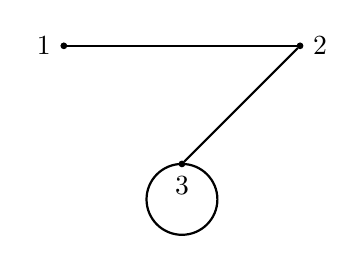
\begin{tikzpicture}[scale=1.5,
    vertex/.style={circle,draw,fill=black,minimum size=2pt,inner sep=0pt}]

\node[vertex,label=left:$1$] (1) at (0,1) {};
\node[vertex,label=right:$2$] (2) at (2,1) {};
\node[vertex,label=below:$3$] (3) at (1,0) {};

\draw[thick] (1) -- (2);
\draw[thick] (2) -- (3);
\draw[thick] (3) ++ (0,-0.3) circle (0.3);
\end{tikzpicture}
\hspace{1cm}
% Right graph (isomorphic)
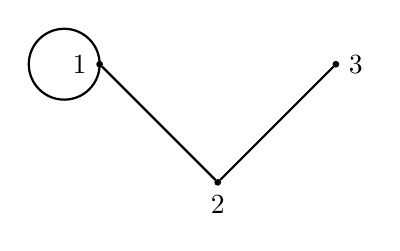
\begin{tikzpicture}[scale=1.5,
    vertex/.style={circle,draw,fill=black,minimum size=2pt,inner sep=0pt}]

\node[vertex,label=left:$1$] (1) at (0,1) {};
\node[vertex,label=below:$2$] (2) at (1,0) {};
\node[vertex,label=right:$3$] (3) at (2,1) {};

\draw[thick] (1) -- (2);
\draw[thick] (2) -- (3);
\draw[thick] (1) ++ (-0.3,0) circle (0.3);
\end{tikzpicture}

\begin{enumerate}[label=(\alph*)]
    \item Give a picture of another graph isomorphic to these two.

    \item Find a graph with vertex set $\{1, 2, 3\}$ that is not isomorphic to the graphs in Figure 3, yet has three edges, exactly one of which is a loop.

    \item Find another example as in part (b) that isn't isomorphic to the one you found in part (b) [or the ones in Figure 3].

    \item Show that $\sim$ is an equivalence relation on the set of all graphs with vertex set $\{1, 2, \ldots, n\}$.
\end{enumerate}
\end{problem}

\begin{proof}[Solution]
~
\begin{enumerate}[label=(\alph*)]
    \item Here is another isomorphic graph, with the loop moved to the middle vertex:

    \begin{center}
    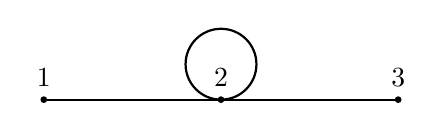
\begin{tikzpicture}[scale=1.5,
        vertex/.style={circle,draw,fill=black,minimum size=2pt,inner sep=0pt}]

    \node[vertex,label=above:$1$] (1) at (0,0) {};
    \node[vertex,label=above:$2$] (2) at (1.5,0) {};
    \node[vertex,label=above:$3$] (3) at (3,0) {};

    \draw[thick] (1) -- (2);
    \draw[thick] (2) -- (3);
    \draw[thick] (2) ++ (0,0.3) circle (0.3);
    \end{tikzpicture}
    \end{center}

    The relabeling $f(1)=1$, $f(2)=3$, $f(3)=2$ maps the loop from vertex 3 to vertex 2. 

    \item Here is a non-isomorphic graph with 3 edges and 1 loop:

    \begin{center}
    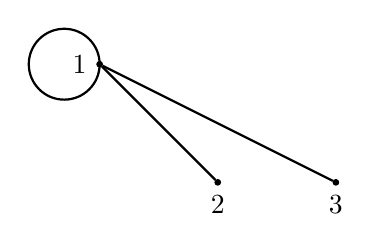
\begin{tikzpicture}[scale=1.5,
        vertex/.style={circle,draw,fill=black,minimum size=2pt,inner sep=0pt}]

    \node[vertex,label=left:$1$] (1) at (0,1) {};
    \node[vertex,label=below:$2$] (2) at (1,0) {};
    \node[vertex,label=below:$3$] (3) at (2,0) {};

    \draw[thick] (1) ++ (-0.3,0) circle (0.3);
    \draw[thick] (1) -- (2);
    \draw[thick] (1) -- (3);
    \end{tikzpicture}
    \end{center}

    1 is connected to 2 and 3 but 2 and 3 are not connected, 1 has a loop. No amount of relabeling can create the graphs in figure 3 or in problem (a).

    \item Another non-isomorphic example:

    \begin{center}
    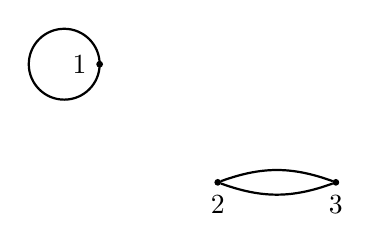
\begin{tikzpicture}[scale=1.5,
        vertex/.style={circle,draw,fill=black,minimum size=2pt,inner sep=0pt}]

    \node[vertex,label=left:$1$] (1) at (0,1) {};
    \node[vertex,label=below:$2$] (2) at (1,0) {};
    \node[vertex,label=below:$3$] (3) at (2,0) {};

    \draw[thick] (1) ++ (-0.3,0) circle (0.3);
    \draw[thick] (2) to[bend left=20] (3);
    \draw[thick] (2) to[bend right=20] (3);
    \end{tikzpicture}
    \end{center}

    Vertex 1 is isolated with only a loop (degree 1), and vertices 2 and 3 are joined by two parallel edges (each with degree 2). This differs from Figure 3 and part (b) since the looped vertex has degree 1 here, not 3.

    \item We check (R), (S), and (T).

    (R): The identity map $f(i) = i$ relabels $G$ to itself, so $G \sim G$.

    (S): If $f$ relabels $G$ to $H$, then $f^{-1}$ (which exists since relabelings are bijections) relabels $H$ back to $G$, so $H \sim G$.

    (T): If $f$ maps $G$ to $H$ and $g$ maps $H$ to $K$, then $g \circ f$ maps $G$ to $K$, so $G \sim K$.

    Therefore $\sim$ is an equivalence relation.
\end{enumerate}
\end{proof}

\setcounter{problem}{7}
\begin{problem}
\begin{enumerate}[label=(\alph*)]
    \item For $m, n \in \ZZ$, define $m \sim n$ in case $m - n$ is odd. Is the relation $\sim$ reflexive? symmetric? transitive? Is $\sim$ an equivalence relation?

    \item For $a$ and $b$ in $\RR$, define $a \sim b$ in case $|a - b| \leq 1$. One could say that $a \sim b$ in case $a$ and $b$ are "close enough" or "approximately equal." Answer the questions in part (a).
\end{enumerate}
\end{problem}

\begin{proof}[Solution]
~
\begin{enumerate}[label=(\alph*)]
    \item (R) fails: $m - m = 0$ is even, so $m \not\sim m$.

    (S) holds: if $m - n$ is odd then $n - m = -(m-n)$ is also odd.

    (T) fails: if $m - n$ and $n - p$ are both odd, their sum $m - p$ is even. For example, $5 - 4 = 1$ (odd) and $4 - 3 = 1$ (odd), but $5 - 3 = 2$ (even).

    So $\sim$ is not an equivalence relation.

    \vspace{0.3in}

    \item (R) holds: $|a - a| = 0 \leq 1$.

    (S) holds: $|b - a| = |a - b| \leq 1$.

    (T) fails: take $a = 0$, $b = 0.9$, $c = 1.8$. Then $|a - b| = 0.9 \leq 1$ and $|b - c| = 0.9 \leq 1$, but $|a - c| = 1.8 > 1$.

    So $\sim$ is not an equivalence relation.
\end{enumerate}
\end{proof}

\setcounter{problem}{9}
\begin{problem}
On the set $\NN \times \NN$ define $(m, n) \sim (k, \ell)$ if $m + \ell = n + k$.

\begin{enumerate}[label=(\alph*)]
    \item Show that $\sim$ is an equivalence relation on $\NN \times \NN$.

    \item Draw a sketch of $\NN \times \NN$ that shows several equivalence classes.
\end{enumerate}
\end{problem}

\begin{proof}[Solution]
~
\begin{enumerate}[label=(\alph*)]
    \item (R): $m + n = n + m$ by commutativity, so $(m,n) \sim (m,n)$.

    (S): if $m + \ell = n + k$, then $k + n = \ell + m$, which is the condition for $(k,\ell) \sim (m,n)$.

    (T): suppose $m + \ell = n + k$ and $k + q = \ell + p$. Adding these gives $m + \ell + k + q = n + k + \ell + p$, and canceling $k + \ell$ from both sides yields $m + q = n + p$, so $(m,n) \sim (p,q)$.

    Therefore $\sim$ is an equivalence relation.

    \vspace{0.3in}

    \item Note that $m + \ell = n + k$ can be rewritten as $m - n = k - \ell$, so two pairs are equivalent when they have the same difference. The equivalence classes are:
    \begin{itemize}
        \item $[(0,0)] = \{(0,0),(1,1),(2,2),\ldots\}$, difference 0
        \item $[(1,0)] = \{(1,0),(2,1),(3,2),\ldots\}$, difference 1
        \item $[(0,1)] = \{(0,1),(1,2),(2,3),\ldots\}$, difference $-1$
    \end{itemize}

    Each class is a diagonal in the $\NN \times \NN$ grid.

    \begin{center}
    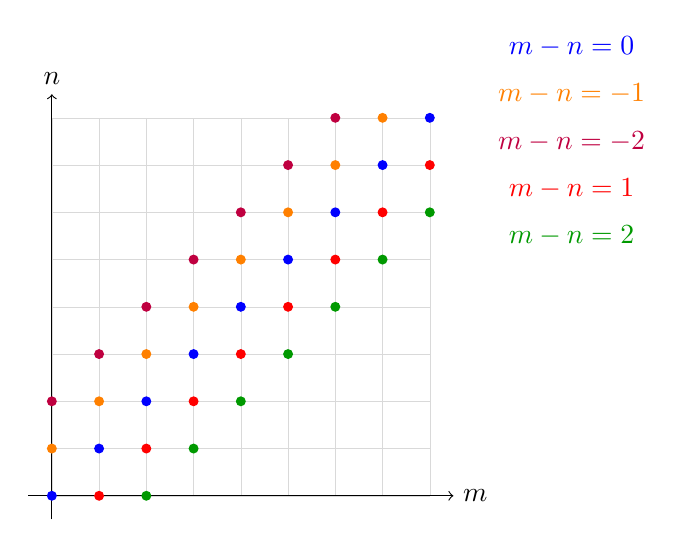
\begin{tikzpicture}[scale=0.6]
    % Grid
    \draw[help lines, gray!30] (0,0) grid (8,8);

    % Axes
    \draw[->] (-0.5,0) -- (8.5,0) node[right] {$m$};
    \draw[->] (0,-0.5) -- (0,8.5) node[above] {$n$};

    % Equivalence class: difference = 0
    \foreach \i in {0,1,2,3,4,5,6,7,8}
        \fill[blue] (\i,\i) circle (3pt);
    \node[blue] at (11,9.5) {$m - n = 0$};

    % Equivalence class: difference = 1
    \foreach \i in {0,1,2,3,4,5,6,7}
        \fill[red] (\i+1,\i) circle (3pt);
    \node[red] at (11,6.5) {$m - n = 1$};

    % Equivalence class: difference = 2
    \foreach \i in {0,1,2,3,4,5,6}
        \fill[green!60!black] (\i+2,\i) circle (3pt);
    \node[green!60!black] at (11,5.5) {$m - n = 2$};

    % Equivalence class: difference = -1
    \foreach \i in {0,1,2,3,4,5,6,7}
        \fill[orange] (\i,\i+1) circle (3pt);
    \node[orange] at (11,8.5) {$m - n = -1$};

    % Equivalence class: difference = -2
    \foreach \i in {0,1,2,3,4,5,6}
        \fill[purple] (\i,\i+2) circle (3pt);
    \node[purple] at (11,7.5) {$m - n = -2$};
    \end{tikzpicture}
    \end{center}
\end{enumerate}
\end{proof}

\setcounter{problem}{16}
\begin{problem}
\begin{enumerate}[label=(\alph*)]
    \item Verify that the relation defined in Example 5(b) is an equivalence relation on $V(G)$.

    \item Given a vertex $v$ in $V(G)$, describe in words the equivalence class containing $v$.
\end{enumerate}

Note: Example 5(b) defines the relation: for vertices $u, v \in V(G)$, $u \sim v$ if there is a path from $u$ to $v$ in $G$.
\end{problem}

\begin{proof}[Solution]
~
\begin{enumerate}[label=(\alph*)]
    \item (R): there is always a trivial path of length 0 from $v$ to itself, so $v \sim v$.

    (S): if there is a path from $u$ to $v$ in an undirected graph, reversing it gives a path from $v$ to $u$, so $v \sim u$.

    (T): if there is a path from $u$ to $v$ and a path from $v$ to $w$, concatenating them gives a path from $u$ to $w$, so $u \sim w$.

    Therefore $\sim$ is an equivalence relation on $V(G)$.

    \vspace{0.3in}

    \item The equivalence class $[v]$ is the set of all vertices reachable from $v$, i.e., the connected component containing $v$. The equivalence classes of this relation are exactly the connected components of $G$.
\end{enumerate}
\end{proof}



    
    Key observations:

\section*{Section 3.5}

\setcounter{problem}{1}
\begin{problem}
Find $n$ DIV $m$ and $n$ MOD $m$ for the following values of $n$ and $m$.

\begin{enumerate}[label=(\alph*)]
    \item $n = 20$, $m = 3$
    \setcounter{enumi}{4}
    
    \item $n = 371{,}246$, $m = 65$
\end{enumerate}
\end{problem}

\begin{proof}[Solution]
~
\begin{enumerate}[label=(\alph*)]
    \item $n = 20$, $m = 3$
    
    By the division algorithm, $20 = 3 \cdot 6 + 2$ where $0 \leq 2 < 3$.
    
    $20$ DIV $3 = 6$ and $20$ MOD $3 = 2$.
    
    \setcounter{enumi}{4}
    
    \item $n = 371{,}246$, $m = 65$
    
    Performing the division: $371{,}246 \div 65 = 5{,}711.477\ldots$
    
    So $q = 5{,}711$ and $r = 371{,}246 - 65 \cdot 5{,}711 = 371{,}246 - 371{,}215 = 31$.
    
    Check: $371{,}246 = 65 \cdot 5{,}711 + 31$ and $0 \leq 31 < 65$.
    
    $371{,}246$ DIV $65 = 5{,}711$ and $371{,}246$ MOD $65 = 31$.
\end{enumerate}
\end{proof}

\setcounter{problem}{3}
\begin{problem}
\begin{enumerate}[label=(\alph*)]
    \item List all equivalence classes of $\ZZ$ for the equivalence relation congruence mod 4.
    
    \item How many different equivalence classes of $\ZZ$ are there with respect to congruence mod 73?
\end{enumerate}
\end{problem}

\begin{proof}[Solution]
~
\begin{enumerate}[label=(\alph*)]
    \item The equivalence classes are determined by the remainder when divided by 4. There are exactly 4 equivalence classes:
    
    \begin{align*}
    [0] &= \{\ldots, -8, -4, 0, 4, 8, 12, \ldots\} = \{4k : k \in \ZZ\} \\
    [1] &= \{\ldots, -7, -3, 1, 5, 9, 13, \ldots\} = \{4k + 1 : k \in \ZZ\} \\
    [2] &= \{\ldots, -6, -2, 2, 6, 10, 14, \ldots\} = \{4k + 2 : k \in \ZZ\} \\
    [3] &= \{\ldots, -5, -1, 3, 7, 11, 15, \ldots\} = \{4k + 3 : k \in \ZZ\}
    \end{align*}
    
    These four classes partition $\ZZ$ since every integer has remainder 0, 1, 2, or 3 when divided by 4.
    
    \item There are exactly \textbf{73 equivalence classes} with respect to congruence mod 73.
    
    The classes are $[0], [1], [2], \ldots, [72]$, where 
    $$[r] = \{73k + r : k \in \ZZ\}$$
    for $r \in \{0, 1, 2, \ldots, 72\}$.
    
    Every integer has a unique remainder in $\{0, 1, 2, \ldots, 72\}$ when divided by 73, so there are exactly 73 distinct equivalence classes.
\end{enumerate}
\end{proof}


\setcounter{problem}{7}
\begin{problem}
\begin{enumerate}[label=(\alph*)]
    \item List the elements in the sets $A_0$, $A_1$, and $A_2$ defined by
    $$A_k = \{m \in \ZZ : -10 < m < 10 \text{ and } m \equiv k \pmod{3}\}.$$
    
    \item What is $A_3$? $A_4$? $A_{73}$?
\end{enumerate}
\end{problem}

\begin{proof}[Solution]
~
\begin{enumerate}[label=(\alph*)]
    \item We need integers in the range $(-10, 10)$ that are congruent to $k$ mod 3.
    
    $A_0$: integers in $(-10, 10)$ with $m \equiv 0 \pmod{3}$
    $$A_0 = \{-9, -6, -3, 0, 3, 6, 9\}$$
    
    $A_1$: integers in $(-10, 10)$ with $m \equiv 1 \pmod{3}$
    $$A_1 = \{-8, -5, -2, 1, 4, 7\}$$
    
    $A_2$: integers in $(-10, 10)$ with $m \equiv 2 \pmod{3}$
    $$A_2 = \{-7, -4, -1, 2, 5, 8\}$$
    
    \item Since congruence mod 3 has only 3 equivalence classes, any integer is congruent to 0, 1, or 2 mod 3.
    
    $A_3$: Since $3 \equiv 0 \pmod{3}$, we have $A_3 = A_0 = \{-9, -6, -3, 0, 3, 6, 9\}$.
    
    $A_4$: Since $4 \equiv 1 \pmod{3}$, we have $A_4 = A_1 = \{-8, -5, -2, 1, 4, 7\}$.
    
    $A_{73}$: Since $73 = 3 \cdot 24 + 1 \equiv 1 \pmod{3}$, we have $A_{73} = A_1 = \{-8, -5, -2, 1, 4, 7\}$.
    
    In general, $A_k = A_{k \bmod 3}$ for any $k \in \ZZ$.
\end{enumerate}
\end{proof}


\setcounter{problem}{11}
\begin{problem}
For $m, n$ in $\NN$, define $m \sim n$ if $m^2 - n^2$ is a multiple of 3.

\begin{enumerate}[label=(\alph*)]
    \item Show that $\sim$ is an equivalence relation on $\NN$.
    
    \item List four elements in the equivalence class $[0]$.
    
    \item List four elements in the equivalence class $[1]$.
    
    \item Do you think there are any more equivalence classes?
\end{enumerate}
\end{problem}

\begin{proof}[Solution]
~
\begin{enumerate}[label=(\alph*)]
    \item (R): $m^2 - m^2 = 0 = 3 \cdot 0$, so $m \sim m$.
    
    (S): if $m^2 - n^2 = 3k$, then $n^2 - m^2 = -(m^2 - n^2) = -3k = 3(-k)$, so $n \sim m$.
    
    (T): if $m^2 - n^2 = 3k$ and $n^2 - p^2 = 3j$, then adding gives $m^2 - p^2 = 3(k + j)$, so $m \sim p$.
    
    Therefore $\sim$ is an equivalence relation.
    
    \item $[0]$ consists of all $n \in \NN$ with $n^2 - 0^2 = n^2$ divisible by 3. This happens when $n^2 \equiv 0 \pmod{3}$, which occurs when $n \equiv 0 \pmod{3}$.
    
    $[0] = \{0, 3, 6, 9, 12, 15, \ldots\}$
    
    Four elements: $0, 3, 6, 9$.
    
    \item $[1]$ consists of all $n \in \NN$ with $n^2 - 1^2 = n^2 - 1$ divisible by 3.
    
    Check: $1^2 - 1 = 0 \equiv 0 \pmod{3}$ (yes), $2^2 - 1 = 3 \equiv 0 \pmod{3}$ (yes), $3^2 - 1 = 8 \equiv 2 \pmod{3}$ (no), $4^2 - 1 = 15 \equiv 0 \pmod{3}$ (yes), $5^2 - 1 = 24 \equiv 0 \pmod{3}$ (yes).
    
    Pattern: $n \in [1]$ when $n^2 \equiv 1 \pmod{3}$, which happens when $n \equiv 1 \pmod{3}$ or $n \equiv 2 \pmod{3}$.
    
    $[1] = \{1, 2, 4, 5, 7, 8, 10, 11, \ldots\}$
    
    Four elements: $1, 2, 4, 5$.
    
    \item No, there are only two equivalence classes: $[0]$ and $[1]$.
    
    For any $n \in \NN$, we have $n \equiv 0, 1,$ or $2 \pmod{3}$.
    
    If $n \equiv 0 \pmod{3}$, then $n^2 \equiv 0 \pmod{3}$, so $n \in [0]$.
    
    If $n \equiv 1 \pmod{3}$, then $n^2 \equiv 1 \pmod{3}$, so $n^2 - 1 \equiv 0 \pmod{3}$, thus $n \in [1]$.
    
    If $n \equiv 2 \pmod{3}$, then $n^2 \equiv 4 \equiv 1 \pmod{3}$, so $n^2 - 1 \equiv 0 \pmod{3}$, thus $n \in [1]$.
    
    Therefore every natural number belongs to either $[0]$ or $[1]$, and these are the only two equivalence classes.
\end{enumerate}
\end{proof}

\section*{Section 11.1}

\setcounter{problem}{0}
\begin{problem}
Draw Hasse diagrams for the following posets.

\begin{enumerate}[label=(\alph*)]
    \item $(\{1, 2, 3, 4, 6, 8, 12, 24\}, \mid)$ where $m \mid n$ means $m$ divides $n$.
    
    \item The set of subsets of $\{3, 7\}$ with $\subseteq$ as partial order.
\end{enumerate}
\end{problem}

\begin{proof}[Solution]
~
\begin{enumerate}[label=(\alph*)]
    \item For the divisibility poset on $\{1, 2, 3, 4, 6, 8, 12, 24\}$:
    
    Covering relations (edges in Hasse diagram):
    \begin{itemize}
        \item 1 is covered by 2 and 3
        \item 2 is covered by 4 and 6
        \item 3 is covered by 6
        \item 4 is covered by 8 and 12
        \item 6 is covered by 12
        \item 8 is covered by 24
        \item 12 is covered by 24
    \end{itemize}
    
    \begin{center}
    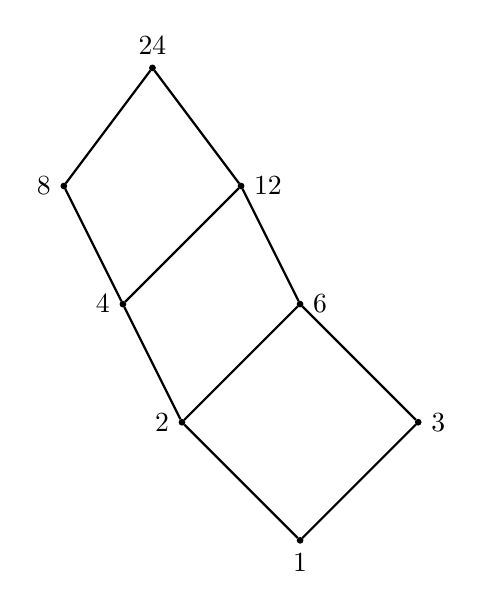
\begin{tikzpicture}[scale=1.5,
        vertex/.style={circle,draw,fill=black,minimum size=2pt,inner sep=0pt}]
    
    % Level 0
    \node[vertex,label=below:$1$] (1) at (0,0) {};
    
    % Level 1
    \node[vertex,label=left:$2$] (2) at (-1,1) {};
    \node[vertex,label=right:$3$] (3) at (1,1) {};
    
    % Level 2
    \node[vertex,label=left:$4$] (4) at (-1.5,2) {};
    \node[vertex,label=right:$6$] (6) at (0,2) {};
    
    % Level 3
    \node[vertex,label=left:$8$] (8) at (-2,3) {};
    \node[vertex,label=right:$12$] (12) at (-0.5,3) {};
    
    % Level 4
    \node[vertex,label=above:$24$] (24) at (-1.25,4) {};
    
    % Edges
    \draw[thick] (1) -- (2);
    \draw[thick] (1) -- (3);
    \draw[thick] (2) -- (4);
    \draw[thick] (2) -- (6);
    \draw[thick] (3) -- (6);
    \draw[thick] (4) -- (8);
    \draw[thick] (4) -- (12);
    \draw[thick] (6) -- (12);
    \draw[thick] (8) -- (24);
    \draw[thick] (12) -- (24);
    \end{tikzpicture}
    \end{center}
    
    \item For the power set of $\{3, 7\}$ ordered by $\subseteq$:
    
    The subsets are: $\emptyset, \{3\}, \{7\}, \{3, 7\}$.
    
    Covering relations:
    \begin{itemize}
        \item $\emptyset$ is covered by $\{3\}$ and $\{7\}$
        \item $\{3\}$ is covered by $\{3, 7\}$
        \item $\{7\}$ is covered by $\{3, 7\}$
    \end{itemize}
    
    \begin{center}
    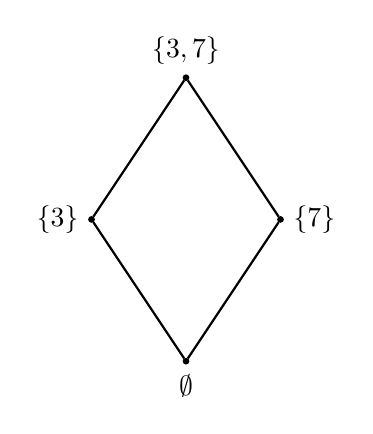
\begin{tikzpicture}[scale=1.5,
        vertex/.style={circle,draw,fill=black,minimum size=2pt,inner sep=0pt}]
    
    % Level 0
    \node[vertex,label=below:$\emptyset$] (e) at (0,0) {};
    
    % Level 1
    \node[vertex,label=left:$\{3\}$] (3) at (-0.8,1.2) {};
    \node[vertex,label=right:$\{7\}$] (7) at (0.8,1.2) {};
    
    % Level 2
    \node[vertex,label={above:$\{3,7\}$}] (37) at (0,2.4) {};
    
    % Edges
    \draw[thick] (e) -- (3);
    \draw[thick] (e) -- (7);
    \draw[thick] (3) -- (37);
    \draw[thick] (7) -- (37);
    \end{tikzpicture}
    \end{center}
\end{enumerate}
\end{proof}

\begin{problem}
Draw a Hasse diagram for $S = \{4, 6, 8, 12\}$ with the partial order $\mid$ (divides).
\end{problem}

\begin{proof}[Solution]
~

Divisibility relations in $S$:
\begin{itemize}
    \item $4 \mid 8$ and $4 \mid 12$
    \item $6 \mid 12$
\end{itemize}

Covering relations (no element between them):
\begin{itemize}
    \item 4 is covered by 8 (since $4 \mid 8$ with no element in $S$ between them)
    \item 4 is covered by 12 (since $4 \mid 12$ with no element in $S$ between them)
    \item 6 is covered by 12
\end{itemize}

Note: 4 and 6 are incomparable (neither divides the other), so they are both minimal elements. Both 8 and 12 are maximal elements.

\begin{center}
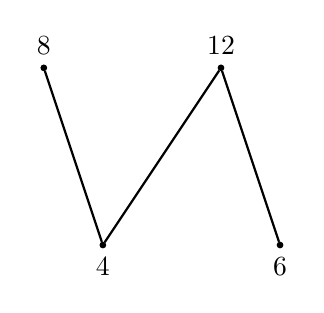
\begin{tikzpicture}[scale=1.5,
    vertex/.style={circle,draw,fill=black,minimum size=2pt,inner sep=0pt}]

% Level 0
\node[vertex,label=below:$4$] (4) at (0,0) {};
\node[vertex,label=below:$6$] (6) at (1.5,0) {};

% Level 1
\node[vertex,label=above:$8$] (8) at (-0.5,1.5) {};
\node[vertex,label=above:$12$] (12) at (1,1.5) {};

% Edges
\draw[thick] (4) -- (8);
\draw[thick] (4) -- (12);
\draw[thick] (6) -- (12);
\end{tikzpicture}
\end{center}
\end{proof}

\setcounter{problem}{14}
\begin{problem}
Define the relations $<$, $\leq$, and $\prec$ on the plane $\RR \times \RR$ by
\begin{align*}
(x,y) < (z,w) &\text{ if } x^2 + y^2 < z^2 + w^2, \\
(x,y) \leq (z,w) &\text{ if } (x,y) < (z,w) \text{ or } (x,y) = (z,w), \\
(x,y) \prec (z,w) &\text{ if } x^2 + y^2 \leq z^2 + w^2.
\end{align*}

\begin{enumerate}[label=(\alph*)]
    \item Which of these relations are partial orders? Explain.
    \setcounter{enumi}{2}
    
    \item Draw a sketch of $\{(x,y) : (x,y) < (3,4)\}$.
    
    \item Draw a sketch of $\{(x,y) : (x,y) \prec (3,4)\}$.
\end{enumerate}
\end{problem}

\begin{proof}[Solution]
~
\begin{enumerate}[label=(\alph*)]
    \item For a partial order, need reflexive, antisymmetric, and transitive.
    
    \textbf{Relation $<$:} Not reflexive since $x^2 + y^2 \not< x^2 + y^2$. Not a partial order.
    
    \textbf{Relation $\leq$:} 
    
    Reflexive: $(x,y) = (x,y)$ always holds.
    
    Antisymmetric: If $(x,y) \leq (z,w)$ and $(z,w) \leq (x,y)$, then we cannot have both $x^2 + y^2 < z^2 + w^2$ and $z^2 + w^2 < x^2 + y^2$. The only possibility is $(x,y) = (z,w)$.
    
    Transitive: If $(x,y) \leq (z,w)$ and $(z,w) \leq (u,v)$, then either some coordinates are equal or we have a chain of strict inequalities, giving $(x,y) \leq (u,v)$.
    
    $\leq$ is a partial order.
    
    \textbf{Relation $\prec$:}
    
    Reflexive: $x^2 + y^2 \leq x^2 + y^2$ always holds.
    
    Antisymmetric: If $(x,y) \prec (z,w)$ and $(z,w) \prec (x,y)$, then $x^2 + y^2 \leq z^2 + w^2$ and $z^2 + w^2 \leq x^2 + y^2$, so $x^2 + y^2 = z^2 + w^2$. But this doesn't imply $(x,y) = (z,w)$ since, e.g., $(3,4)$ and $(4,3)$ both satisfy $x^2 + y^2 = 25$. Not antisymmetric.
    
    $\prec$ is not a partial order.
    
    \textbf{Answer:} Only $\leq$ is a partial order.
    
    \setcounter{enumi}{2}
    
    \item $\{(x,y) : (x,y) < (3,4)\} = \{(x,y) : x^2 + y^2 < 25\}$

    This is the open disk of radius 5 centered at the origin.

    \begin{center}
    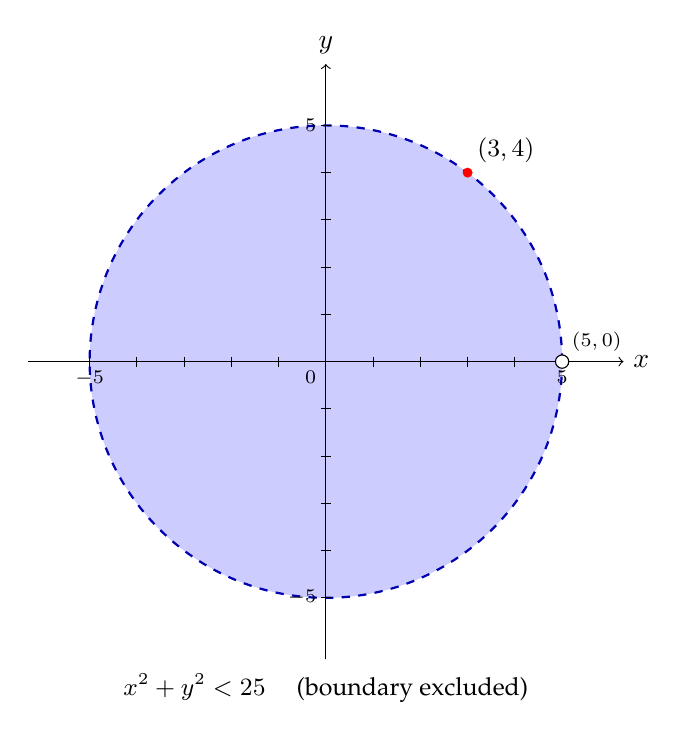
\begin{tikzpicture}[scale=0.6]
    % Open disk (shaded, dashed boundary means excluded)
    \fill[blue!20] (0,0) circle (5);
    \draw[dashed, thick, blue!70!black] (0,0) circle (5);

    % Axes (drawn after fill so they appear on top)
    \draw[->] (-6.3,0) -- (6.3,0) node[right] {$x$};
    \draw[->] (0,-6.3) -- (0,6.3) node[above] {$y$};

    % Tick marks
    \foreach \x in {-5,-4,-3,-2,-1,1,2,3,4,5}
        \draw (\x,3pt) -- (\x,-3pt);
    \foreach \y in {-5,-4,-3,-2,-1,1,2,3,4,5}
        \draw (3pt,\y) -- (-3pt,\y);

    % Axis labels at key values
    \node[below, font=\scriptsize] at ( 5, 0) {$5$};
    \node[below, font=\scriptsize] at (-5, 0) {$-5$};
    \node[left,  font=\scriptsize] at ( 0, 5) {$5$};
    \node[left,  font=\scriptsize] at ( 0,-5) {$-5$};
    \node[below left, font=\scriptsize] at (0,0) {$0$};

    % Reference point (3,4) — on the boundary circle
    \fill[red] (3,4) circle (3pt);
    \node[above right, font=\small] at (3,4) {$(3,4)$};

    % Open boundary indicator at (5,0)
    \fill[white] (5,0) circle (4pt);
    \draw (5,0) circle (4pt);
    \node[above right, font=\scriptsize] at (5,0) {$(5,0)$};

    % Caption
    \node[below, font=\small] at (0,-6.4) {$x^2+y^2 < 25$ \quad (boundary excluded)};
    \end{tikzpicture}
    \end{center}

    \item $\{(x,y) : (x,y) \prec (3,4)\} = \{(x,y) : x^2 + y^2 \leq 25\}$

    This is the closed disk of radius 5 centered at the origin.

    \begin{center}
    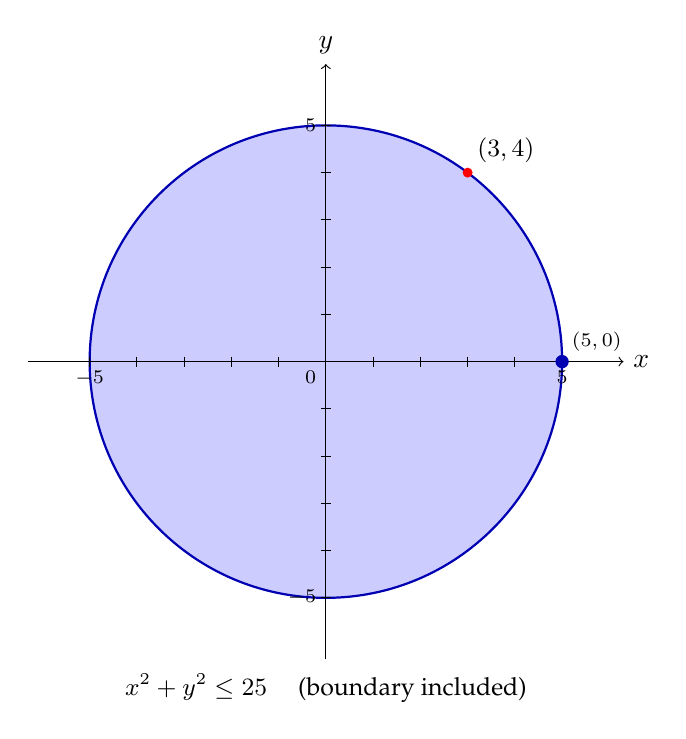
\begin{tikzpicture}[scale=0.6]
    % Closed disk (shaded, solid boundary means included)
    \fill[blue!20] (0,0) circle (5);
    \draw[thick, blue!70!black] (0,0) circle (5);

    % Axes (drawn after fill so they appear on top)
    \draw[->] (-6.3,0) -- (6.3,0) node[right] {$x$};
    \draw[->] (0,-6.3) -- (0,6.3) node[above] {$y$};

    % Tick marks
    \foreach \x in {-5,-4,-3,-2,-1,1,2,3,4,5}
        \draw (\x,3pt) -- (\x,-3pt);
    \foreach \y in {-5,-4,-3,-2,-1,1,2,3,4,5}
        \draw (3pt,\y) -- (-3pt,\y);

    % Axis labels at key values
    \node[below, font=\scriptsize] at ( 5, 0) {$5$};
    \node[below, font=\scriptsize] at (-5, 0) {$-5$};
    \node[left,  font=\scriptsize] at ( 0, 5) {$5$};
    \node[left,  font=\scriptsize] at ( 0,-5) {$-5$};
    \node[below left, font=\scriptsize] at (0,0) {$0$};

    % Reference point (3,4) — on the boundary circle
    \fill[red] (3,4) circle (3pt);
    \node[above right, font=\small] at (3,4) {$(3,4)$};

    % Closed boundary indicator at (5,0)
    \fill[blue!70!black] (5,0) circle (4pt);
    \node[above right, font=\scriptsize] at (5,0) {$(5,0)$};

    % Caption
    \node[below, font=\small] at (0,-6.4) {$x^2+y^2 \leq 25$ \quad (boundary included)};
    \end{tikzpicture}
    \end{center}
\end{enumerate}
\end{proof}

\section*{Section 11.2}

\setcounter{problem}{8}
\begin{problem}
Let $S = \{0, 1, 2\}$ with the usual order, and let $T = \{a, b\}$ with $a < b$.

\begin{enumerate}[label=(\alph*)]
    \setcounter{enumi}{1}
    \item Draw a Hasse diagram for the poset $(S \times S, \prec)$ with the product order.
    
    \item Draw a Hasse diagram for $S \times T$ with the product order.
\end{enumerate}
\end{problem}

\begin{proof}[Solution]
~
\begin{enumerate}[label=(\alph*)]
    \setcounter{enumi}{1}
    \item For the product order on $S \times S$ where $S = \{0, 1, 2\}$: $(a,b) \prec (c,d)$ if $a \leq c$ and $b \leq d$.
    
    Elements: $(0,0), (0,1), (0,2), (1,0), (1,1), (1,2), (2,0), (2,1), (2,2)$
    
    \begin{center}
    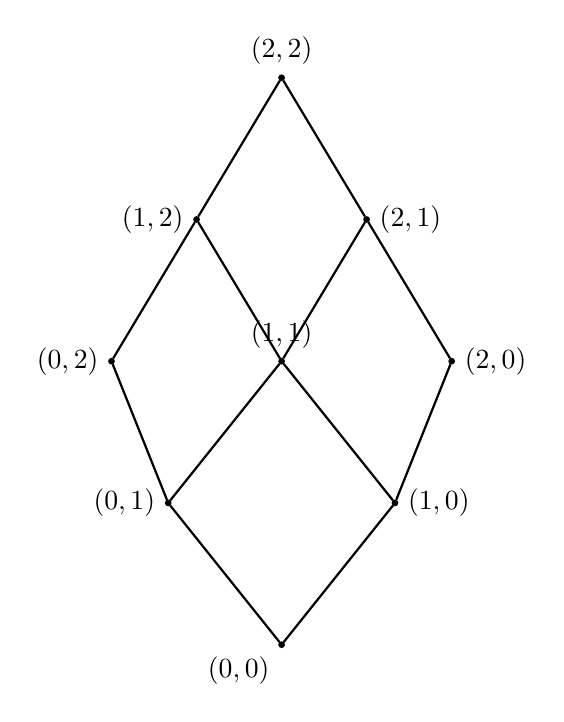
\begin{tikzpicture}[scale=1.8,
        vertex/.style={circle,draw,fill=black,minimum size=2pt,inner sep=0pt}]
    
    % Level 0
    \node[vertex,label={below left:$(0,0)$}] (00) at (0,0) {};

    % Level 1
    \node[vertex,label={left:$(0,1)$}] (01) at (-0.8,1) {};
    \node[vertex,label={right:$(1,0)$}] (10) at (0.8,1) {};

    % Level 2
    \node[vertex,label={left:$(0,2)$}] (02) at (-1.2,2) {};
    \node[vertex,label={above:$(1,1)$}] (11) at (0,2) {};
    \node[vertex,label={right:$(2,0)$}] (20) at (1.2,2) {};

    % Level 3
    \node[vertex,label={left:$(1,2)$}] (12) at (-0.6,3) {};
    \node[vertex,label={right:$(2,1)$}] (21) at (0.6,3) {};

    % Level 4
    \node[vertex,label={above:$(2,2)$}] (22) at (0,4) {};
    
    % Edges
    \draw[thick] (00) -- (01);
    \draw[thick] (00) -- (10);
    \draw[thick] (01) -- (02);
    \draw[thick] (01) -- (11);
    \draw[thick] (10) -- (11);
    \draw[thick] (10) -- (20);
    \draw[thick] (02) -- (12);
    \draw[thick] (11) -- (12);
    \draw[thick] (11) -- (21);
    \draw[thick] (20) -- (21);
    \draw[thick] (12) -- (22);
    \draw[thick] (21) -- (22);
    \end{tikzpicture}
    \end{center}
    
    \item For $S \times T$ with product order where $S = \{0,1,2\}$ and $T = \{a,b\}$: $(s_1, t_1) \prec (s_2, t_2)$ if $s_1 \leq s_2$ and $t_1 \leq t_2$ (where $a < b$).
    
    Elements: $(0,a), (0,b), (1,a), (1,b), (2,a), (2,b)$
    
    \begin{center}
    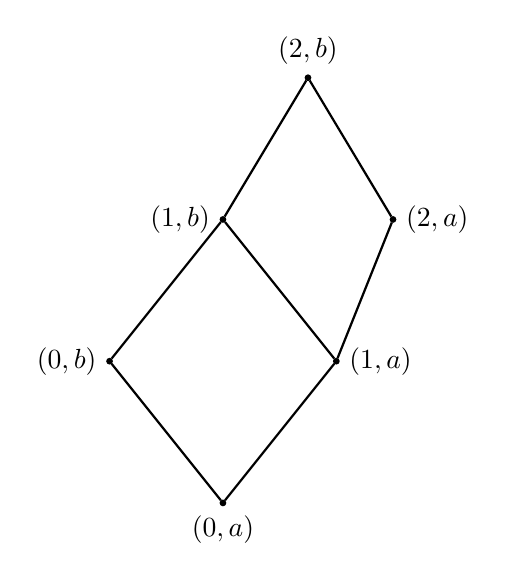
\begin{tikzpicture}[scale=1.8,
        vertex/.style={circle,draw,fill=black,minimum size=2pt,inner sep=0pt}]
    
    % Level 0
    \node[vertex,label={below:$(0,a)$}] (0a) at (0,0) {};

    % Level 1
    \node[vertex,label={left:$(0,b)$}] (0b) at (-0.8,1) {};
    \node[vertex,label={right:$(1,a)$}] (1a) at (0.8,1) {};

    % Level 2
    \node[vertex,label={left:$(1,b)$}] (1b) at (0,2) {};
    \node[vertex,label={right:$(2,a)$}] (2a) at (1.2,2) {};

    % Level 3
    \node[vertex,label={above:$(2,b)$}] (2b) at (0.6,3) {};
    
    % Edges
    \draw[thick] (0a) -- (0b);
    \draw[thick] (0a) -- (1a);
    \draw[thick] (0b) -- (1b);
    \draw[thick] (1a) -- (1b);
    \draw[thick] (1a) -- (2a);
    \draw[thick] (1b) -- (2b);
    \draw[thick] (2a) -- (2b);
    \end{tikzpicture}
    \end{center}
\end{enumerate}
\end{proof}

\begin{problem}
Draw a Hasse diagram for $S \times T$, where $S = \{4, 6, 8, 12\}$ with the partial order $\mid$ (divides), and $T = \{2, 3, 5\}$ with the partial order $\leq$.

\begin{enumerate}[label=(\alph*)]
    \item the product order
    
    \item the lexicographic order
\end{enumerate}
\end{problem}

\begin{proof}[Solution]
~
\begin{enumerate}[label=(\alph*)]
    \item For the product order: $(s_1, t_1) \prec (s_2, t_2)$ if $s_1 \mid s_2$ and $t_1 \leq t_2$.
    
    Recall from Section 11.1 that in $S$: $4 \mid 8$, $4 \mid 12$, $6 \mid 12$, and 4, 6 are incomparable.
    
    Elements of $S \times T$: $(4,2), (4,3), (4,5), (6,2), (6,3), (6,5), (8,2), (8,3), (8,5), (12,2), (12,3), (12,5)$
    
    \begin{center}
    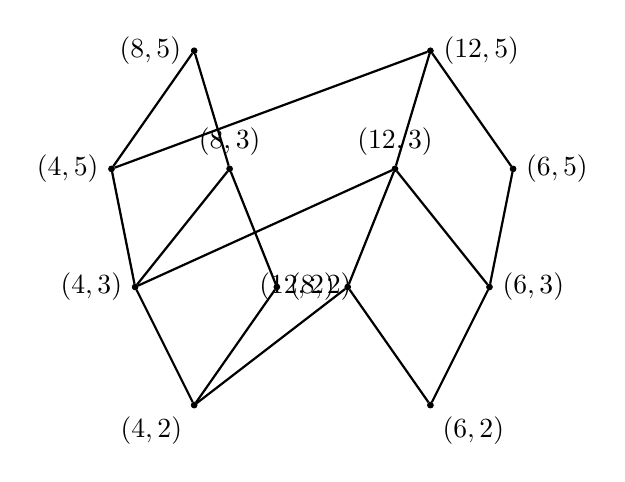
\begin{tikzpicture}[scale=1.5,
        vertex/.style={circle,draw,fill=black,minimum size=2pt,inner sep=0pt}]
    
    % Bottom level
    \node[vertex,label={below left:$(4,2)$}] (42) at (0,0) {};
    \node[vertex,label={below right:$(6,2)$}] (62) at (2,0) {};

    % Level 1
    \node[vertex,label={left:$(4,3)$}] (43) at (-0.5,1) {};
    \node[vertex,label={right:$(8,2)$}] (82) at (0.7,1) {};
    \node[vertex,label={left:$(12,2)$}] (122) at (1.3,1) {};
    \node[vertex,label={right:$(6,3)$}] (63) at (2.5,1) {};

    % Level 2
    \node[vertex,label={left:$(4,5)$}] (45) at (-0.7,2) {};
    \node[vertex,label={above:$(8,3)$}] (83) at (0.3,2) {};
    \node[vertex,label={above:$(12,3)$}] (123) at (1.7,2) {};
    \node[vertex,label={right:$(6,5)$}] (65) at (2.7,2) {};

    % Level 3
    \node[vertex,label={left:$(8,5)$}] (85) at (0,3) {};
    \node[vertex,label={right:$(12,5)$}] (125) at (2,3) {};
    
    % Edges from (4,2)
    \draw[thick] (42) -- (43);
    \draw[thick] (42) -- (82);
    \draw[thick] (42) -- (122);
    
    % Edges from (6,2)
    \draw[thick] (62) -- (63);
    \draw[thick] (62) -- (122);
    
    % Edges from (4,3)
    \draw[thick] (43) -- (45);
    \draw[thick] (43) -- (83);
    \draw[thick] (43) -- (123);
    
    % Edges from (8,2)
    \draw[thick] (82) -- (83);
    
    % Edges from (12,2)
    \draw[thick] (122) -- (123);
    
    % Edges from (6,3)
    \draw[thick] (63) -- (65);
    \draw[thick] (63) -- (123);
    
    % Edges from (4,5)
    \draw[thick] (45) -- (85);
    \draw[thick] (45) -- (125);
    
    % Edges from (8,3)
    \draw[thick] (83) -- (85);
    
    % Edges from (12,3)
    \draw[thick] (123) -- (125);
    
    % Edges from (6,5)
    \draw[thick] (65) -- (125);
    \end{tikzpicture}
    \end{center}
    
    \item For the lexicographic order: $(s_1, t_1) \prec (s_2, t_2)$ if $s_1 \mid s_2$ and $s_1 \neq s_2$, OR $s_1 = s_2$ and $t_1 < t_2$.
    
    The lexicographic order first compares using the divisibility relation on $S$, then breaks ties using $\leq$ on $T$.
    \begin{itemize}
        \item All pairs with first coordinate 4 come before pairs with 8 or 12 (since $4 \mid 8$ and $4 \mid 12$)
        \item All pairs with first coordinate 6 come before pairs with 12 (since $6 \mid 12$)
        \item Pairs with 4 and pairs with 6 are incomparable (different chains)
        \item Within same first coordinate, order by second coordinate
    \end{itemize}
    
    \begin{center}
    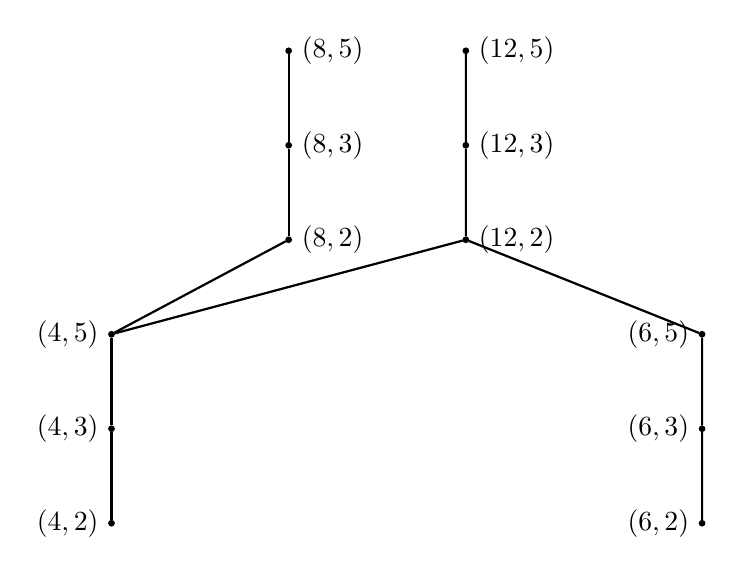
\begin{tikzpicture}[scale=1.5,
        vertex/.style={circle,draw,fill=black,minimum size=2pt,inner sep=0pt}]
    
    % Chain starting with 4
    \node[vertex,label={left:$(4,2)$}] (42) at (0,0) {};
    \node[vertex,label={left:$(4,3)$}] (43) at (0,0.8) {};
    \node[vertex,label={left:$(4,5)$}] (45) at (0,1.6) {};

    \node[vertex,label={right:$(8,2)$}] (82) at (1.5,2.4) {};
    \node[vertex,label={right:$(8,3)$}] (83) at (1.5,3.2) {};
    \node[vertex,label={right:$(8,5)$}] (85) at (1.5,4) {};

    \node[vertex,label={right:$(12,2)$}] (122) at (3,2.4) {};
    \node[vertex,label={right:$(12,3)$}] (123) at (3,3.2) {};
    \node[vertex,label={right:$(12,5)$}] (125) at (3,4) {};

    % Chain starting with 6
    \node[vertex,label={left:$(6,2)$}] (62) at (5,0) {};
    \node[vertex,label={left:$(6,3)$}] (63) at (5,0.8) {};
    \node[vertex,label={left:$(6,5)$}] (65) at (5,1.6) {};
    
    % Edges in 4 chain
    \draw[thick] (42) -- (43);
    \draw[thick] (43) -- (45);
    
    % Edges from 4 to 8
    \draw[thick] (45) -- (82);
    
    % Edges in 8 chain
    \draw[thick] (82) -- (83);
    \draw[thick] (83) -- (85);
    
    % Edges from 4 to 12
    \draw[thick] (45) -- (122);
    
    % Edges in 12 chain
    \draw[thick] (122) -- (123);
    \draw[thick] (123) -- (125);
    
    % Edges in 6 chain
    \draw[thick] (62) -- (63);
    \draw[thick] (63) -- (65);
    
    % Edges from 6 to 12
    \draw[thick] (65) -- (122);
    \end{tikzpicture}
    \end{center}
\end{enumerate}
\end{proof}


\end{document}
